
\begin{frame}{Matrix-Vector Multiplication}
\begin{itemize}
    \item The product of an $m\times n$ matrix $A$ and an $n$-dimensional vector $x$ yields an $m$-dimensional vector $y = Ax$, where each entry is computed as:
    \begin{align*}
        y_i = A_{i1}x_1 + \cdots + A_{in}x_n, \; i=1, \ldots, m
    \end{align*}
    
\end{itemize} 
\end{frame}

\begin{frame}{}
\begin{figure}[h]
    \begin{center}
    \begin{tikzpicture}[baseline=(current bounding box.center)]
        % Matrix (A)
        \node at (0,0) {
        $\begin{bmatrix}
        \colorbox{green!30}{$a_{11}$} & \colorbox{green!30}{$a_{12}$} & \colorbox{green!30}{$a_{13}$} \\
        a_{21} & a_{22} & a_{23} \\
        a_{31} & a_{32} & a_{33}
        \end{bmatrix}$
        };

        % Vector (x)  
        \node at (3,0) {
        $\begin{bmatrix}
        \colorbox{green!30}{$x_1$} \\
        \colorbox{green!30}{$x_2$} \\
        \colorbox{green!30}{$x_3$}
        \end{bmatrix}$
        };

        % Equals sign
        \node at (4.2,0) {$=$};

        % Result vector (b)
        \node at (5.5,0) {
        $\begin{bmatrix}
        \colorbox{blue!30}{$y_1$} \\
        y_2 \\
        y_3
        \end{bmatrix}$
        };
    \end{tikzpicture}
    \caption{Computing the first element $y_1 = a_{11}x_1 + a_{12}x_2 + a_{13}x_3$}
    \label{fig:matrix-vector-multiplication}
    \end{center}
\end{figure}
\begin{itemize}
    \item This operation can be viewed as computing dot products between matrix rows and the vector:
    \begin{align}
        y_i= a_i^T x, \; i=1, \ldots, m
    \end{align}
    where $a^T_1, \ldots, a^T_m$ denote the rows of matrix $A$, i.e., $a_i^T = [A_{i1}, A_{i2}, \ldots, A_{in}]$.
\end{itemize}
\end{frame}

\begin{frame}
    \begin{itemize}
        \item Example:
            \begin{align*}
                \begin{bmatrix}
                    0 & 2 & -1\\
                    -1 & 1 & 0 
                \end{bmatrix}\begin{bmatrix}
                    1\\
                    2\\
                    -1
                \end{bmatrix} & = \begin{bmatrix}
                    0 \cdot 1 + 2 \cdot 2 + (-1) \cdot (-1)\\
                    (-1) \cdot 1 + 1 \cdot 2 + 0 \cdot (-1)
                \end{bmatrix}\\
                &  = \begin{bmatrix}
                    0 + 4 + 1\\
                    -1 + 2 + 0
                \end{bmatrix} \\
               &  = \begin{bmatrix}
                    5\\
                    1
                \end{bmatrix}
            \end{align*}
    
    \end{itemize}
\end{frame}



\begin{frame}{Special Cases and Alternative Interpretation}
\begin{itemize}
    \item When multiplying matrix $A$ by the vector of ones $\boldsymbol{1}$, the result is a vector containing the row sums of $A$:
    \begin{align*}
        \begin{bmatrix}
            0 & 2 & -1\\
            -1 & 1 & 0 
        \end{bmatrix}\begin{bmatrix}
            1\\
            1\\
            1\\
        \end{bmatrix} = \begin{bmatrix}
            0 + 2 + (-1)\\
            -1 + 1 + 0 
        \end{bmatrix} = \begin{bmatrix}
            1\\0
        \end{bmatrix}
    \end{align*}
    \item The matrix-vector product $y=Ax$ can alternatively be expressed as:
    \begin{align*}
        y = x_1 a_1 + \cdots + x_n a_n
    \end{align*}
    where $a_1, \ldots, a_n$ represent the columns of matrix $A$.
\end{itemize}
\end{frame}
\begin{frame}
    \begin{itemize}
        \item This interpretation shows that $y=Ax$ is a linear combination of the columns of $A$, with weights given by the components $x_1, \ldots, x_n$.
    \end{itemize}
\end{frame}



\begin{frame}{Matrix Multiplication}
\begin{itemize}
    \item For matrices $A$ (dimensions $n \times m$) and $B$ (dimensions $p \times q$)
    \item The matrix product $C = AB$ is defined if and only if the number of columns in $A$ equals the number of rows in $B$, i.e., $m = p$
    \item When this condition is satisfied, the resulting matrix $C$ has dimensions $n \times q$, with elements computed as:
    \begin{align}
        C_{ij} = \sum_{k=1}^m A_{ik} B_{kj}
    \end{align}
    \item The product $AB$ is obtained by computing the dot product of each row of $A$ with each column of $B$
\end{itemize}    
\end{frame}



\begin{frame}{}
\begin{itemize}
    \item Equivalently, the matrix product can be expressed as:
    \begin{align}
        C = \begin{bmatrix}
            a_1^T\\
            a_2^T\\
            \vdots\\
            a_n^T
        \end{bmatrix}\begin{bmatrix}
            b_1 & b_2 & \cdots & b_q
        \end{bmatrix} = \begin{bmatrix}
            a_1^T b_1 & a_1^T b_2 & \cdots & a_1^T b_q\\
            a_2^T b_1 & a_2^T b_2 & \cdots & a_2^T b_q\\
            \vdots & \vdots & \ddots & \vdots\\
            a_n^T b_1 & a_n^T b_2 & \cdots & a_n^T b_q
        \end{bmatrix}
    \end{align}
    where $a_i^T$ denotes the $i$-th row of matrix $A$ and $b_j$ represents the $j$-th column of matrix $B$.
\end{itemize}
\end{frame}

\begin{frame}{}
    \begin{figure}
        \begin{center}
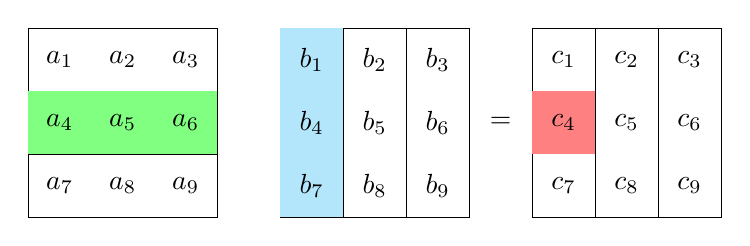
\begin{tikzpicture}[scale=0.8]
    % Matrix A
    \draw (0,0) rectangle (3,3);
    \draw (0,2) rectangle (3,3);
    \fill[green!50] (0,1) rectangle (3,2);
    \draw (0,0) rectangle (3,1);
    
    \node at (0.5,2.5) {$a_1$};
    \node at (1.5,2.5) {$a_2$};
    \node at (2.5,2.5) {$a_3$};
    \node at (0.5,1.5) {$a_4$};
    \node at (1.5,1.5) {$a_5$};
    \node at (2.5,1.5) {$a_6$};
    \node at (0.5,0.5) {$a_7$};
    \node at (1.5,0.5) {$a_8$};
    \node at (2.5,0.5) {$a_9$};
    
    % Matrix B
    \draw (4,0) rectangle (7,3);
    \fill[cyan!30] (4,0) rectangle (5,3);
    \draw (5,0) rectangle (6,3);
    \draw (6,0) rectangle (7,3);
    
    \node at (4.5,2.5) {$b_1$};
    \node at (5.5,2.5) {$b_2$};
    \node at (6.5,2.5) {$b_3$};
    \node at (4.5,1.5) {$b_4$};
    \node at (5.5,1.5) {$b_5$};
    \node at (6.5,1.5) {$b_6$};
    \node at (4.5,0.5) {$b_7$};
    \node at (5.5,0.5) {$b_8$};
    \node at (6.5,0.5) {$b_9$};
    
    % Equals sign
    \node at (7.5,1.5) {$=$};
    
    % Result matrix C
    \draw (8,0) rectangle (11,3);

    \fill[red!50] (8,2) rectangle (9,1);
    \draw (9,0) rectangle (10,3);
    \draw(10,0) rectangle (11,3);
    
    % \draw(4.5,0) rectangle (8.5,2.5);

    \node at (8.5,2.5) {$c_1$};
    \node at (9.5,2.5) {$c_2$};
    \node at (10.5,2.5) {$c_3$};
    \node at (8.5,1.5) {$c_4$};
    \node at (9.5,1.5) {$c_5$};
    \node at (10.5,1.5) {$c_6$};
    \node at (8.5,0.5) {$c_7$};
    \node at (9.5,0.5) {$c_8$};
    \node at (10.5,0.5) {$c_9$};
    
\end{tikzpicture}
        \caption{Matrix multiplication visualization}
        \label{fig:matrix_multiplication}
\end{center}
\end{figure}
\end{frame}

\begin{frame}{Matrix Multiplication Example}
\begin{itemize}
    \item Consider matrices $A$ and $B$:
    \begin{align*}
        A = \begin{bmatrix}
            1 & 2 & 3\\
            4 & 5 & 6
        \end{bmatrix}, \quad B = \begin{bmatrix}    
            7 & 8\\
            9 & 10\\
            11 & 12
        \end{bmatrix}
    \end{align*}
    \item The product $C = AB$ is computed as follows:
    \begin{align*}
        C_{11} = 1 \cdot 7 + 2 \cdot    9 + 3 \cdot 11 = 58, \quad
        C_{12} = 1 \cdot 8 + 2 \cdot 10 + 3 \cdot 12 = 64\\
        C_{21} = 4 \cdot 7 + 5 \cdot 9 + 6 \cdot 11 = 139, \quad
        C_{22} = 4 \cdot 8 + 5 \cdot 10 + 6 \cdot 12 = 154
    \end{align*}
\end{itemize}
\end{frame}

\begin{frame}
    \begin{itemize}
        \item Thus, the resulting matrix $C$ is:
    \begin{align*}  
        C = \begin{bmatrix}
            58 & 64\\
            139 & 154
        \end{bmatrix}
    \end{align*}
        \item Note that matrix multiplication is not commutative, i.e., $AB \neq BA$ in general
        \item However, it is associative, i.e., $(AB)C = A(BC)$
        \item It is also distributive over addition, i.e., $A(B + C) = AB + AC$
        \item The identity matrix $I_n$ serves as the multiplicative identity for matrices, i.e., $AI_n = A$ and $I_nA = A$ for any compatible matrix $A$
        \item The zero matrix $O$ acts as the additive identity, satisfying $A + O = A$ and $O + A = A$ for any matrix $A$
    \end{itemize}
\end{frame}